\begin{voorstel}{Geothermie}
\meeschrijver{Rints Swart}

\begin{samenvatting}
Samenvatting
\end{samenvatting}

\begin{uitdaging}
Op diverse plekken in Nederland wordt aardwarmte met succes gebruikt voor de verwarming van kassen. De eerste aardwarmtewinning is in 2007 in Bleiswijk gerealiseerd. Verwarming van een kas met water van 60 graden Celsius afkomstig van 1700 meter diepte. .(Bron: Bosatlas van de Energie)

In Zwolle wordt in het kader van de energietransitie onderzoek gedaan naar de toepassing van geothermie voor de verwarming van reeds bestaande stadswijken, Holtenbroek en Aalanden.

Op deze schaalgrootte is dat in Nederland nog niet eerder onderzocht en toegepast.

In Frankrijk wordt al tientallen jaren zonder problemen warmte uit de aarde gebruikt voor woonwijken in de regio van  Parijs (zie: Geothermie en Ile-de-France en Geothermie a Villages Nature Paris).

De rijksoverheid (Planbureau voor de Leefomgeving) geeft op basis van de uitkomsten van het SCAN-onderzoek aan waar in Nederland geschikte locaties zijn om, gebruik makend van geothermische warmte, stadswijken te voorzien van warmte. (Zo ook bijvoorbeeld voor de stad Groningen). In 2022 zou een eerste landelijk beeld gegeven kunnen worden (Regie bij het Rijk).
\end{uitdaging}

\begin{overwegingen}
\paragraph{Uitleg aardwarmte}
Wat is aardwarmte en welke typen warmte onderscheiden we: geothermie, diepe geothermie en ultra diepe geothermie. 

Hoe dieper we de warmte oppompen hoe warmer het water is.

Voor verwarming van woningen en kantoren is een warmte van 45 graden Celsius voldoende.

Voor de glastuinbouw wordt 70 graden op prijs gesteld. 
Voor de industrie …

Water van meer dan 100 graden kan een elektrische centrale bedienen.

Daarnaast is uitleg van WKO-systemen (warmte-koude opslag) verstandig (www.wkotool.nl).

Er is al veel bekend over de ondergrond van Nederland met watervoerende aardlagen ( zie kaarten van 2 km diepte en 5 km diepte.

Momenteel vindt seismisch onderzoek plaats om ontbrekende gedeelten van de ondergrond nauwkeuriger in beeld te krijgen: SCAN = Seismische Campagne Aardwarmte Nederland.

In de glastuinbouw worden goede resultaten behaald: Bleiswijk, Koekoekspolder (IJsselmuiden).

In Zwolle wordt in het kader van de Regionale Energie Strategie (RES) een pilot-project uitgevoerd voor de verwarming van bestaande woonwijken. Een proefboring zal volgend jaar plaatsvinden.

In eerste instantie zijn proefboringen een dure aangelegenheid omdat roestvrijstalen buizen nodig zijn. Er zijn per locatie twee buizen nodig om het warme water op te pompen en daarna via een andere buis terug te pompen.

In tegenstelling tot de winning van schaliegas vindt nauwelijks verontreiniging van de ondergrond plaats. Bij de winning van schaliegas is het grote probleem dat het verontreinigde water eerst in basins weer schoongemaakt moet worden. Bovendien wordt daarbij met explosies de gasvoerende lagen gebroken. Bij aardwarmte gaat het om goed watervoerende lagen die afgedekt zijn door ondoorlatende kleilagen. In de buizen worden kleine pompen aangebracht die op zich energie behoeven, elektriciteit). Bij de projecten voor de glastuinbouw is gebleken dat de daarvoor benodigde energie ruimschoots de besparende elektriciteit door de warmtewisselaar overtreft. In het opgepompte water wordt wel zout gewonnen.

De warmtenetten bij de glastuinbouw zijn van korte lengte, wat bij grote woningbouwprojecten niet het geval is. Bij glastuinbouw is het een gezamenlijk initiatief van ondernemende tuinders..Voor de proefboringen is het de overheid die dat grotendeels financiert. Bij de Koekoekspolder is dat de provincie Overijssel. Na enkele problemen is er nu zelfs sprake van uitbreiding van het aantal hectare kassen. In het geval van een complete woonwijk is het de gemeente die aanvankelijk de regie voert. Daarbij wordt ze bijgestaan door deskundigen van EBN, TNO en adviesbureaus.

Bij de glastuinbouw is gebleken dat de kosten van boringen en continue energie voor pompen e.d. op termijn terugverdiend kunnen worden.

Geothermie in de glastuinbouw stimuleren.
Voor de verwarming van stadswijken verder onderzoek doen en toepassen.

\paragraph{Uitleg}
De hete kern van de aarde is een vrijwel onuitputtelijke bron van aardwarmte. Op 2 kilometer diepte heeft grondwater in Nederland gemiddeld al een temperatuur van meer dan 70 graden Celsius. Met opgepompt grondwater van meer dan 45 graden C kun je huizen en kassen verwarmen, boven de 120 graden Celsius kun je mogelijk elektriciteit opwekken. De potentie voor de winning van aardwarmte is o.a. afhankelijk van de temperatuur van het grondwater, de dikte en doorlatendheid van de watervoerende laag.

\paragraph{Geothermie in de tuinbouw}
Voor verwarming van tuinbouwkassen zijn reeds diverse voorbeelden te noemen, waaronder in de Koekoekspolder bij IJsselmuiden.

\paragraph{Verwarming woonwijken}
Het project in Zwolle is een van de eerste grootschalige toepassingen van geothermie voor de verwarming van bestaande woonwijken. Het is een pilot-project en de ervaringen die ermee worden opgedaan kunnen elders in Nederland van nut zijn. Het succes hangt af van de ligging van warm water in de aardlagen onder de plek waar de warmte gebruikt wordt.

Geologisch onderzoek van de bodem in Nederland heeft reeds een beeld opgeleverd dat toepassing van aardwarmte mogelijk maakt. Zie kaarten:

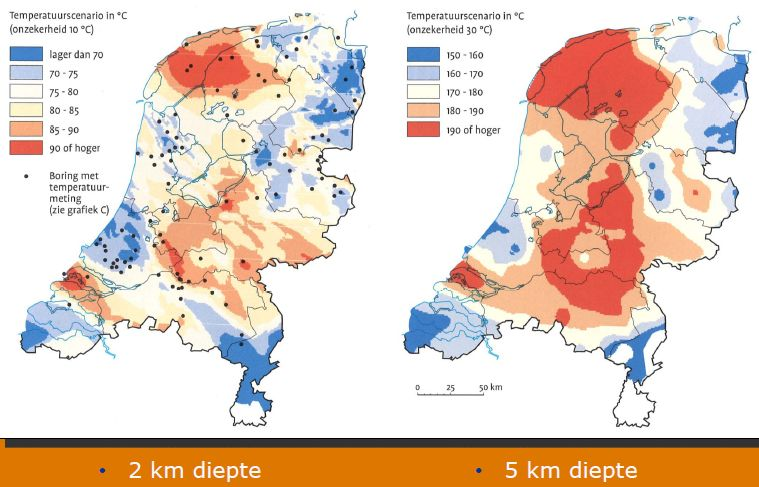
\includegraphics[width=.5\textwidth]{img/energie/geothermie-temperatuurscenarios}
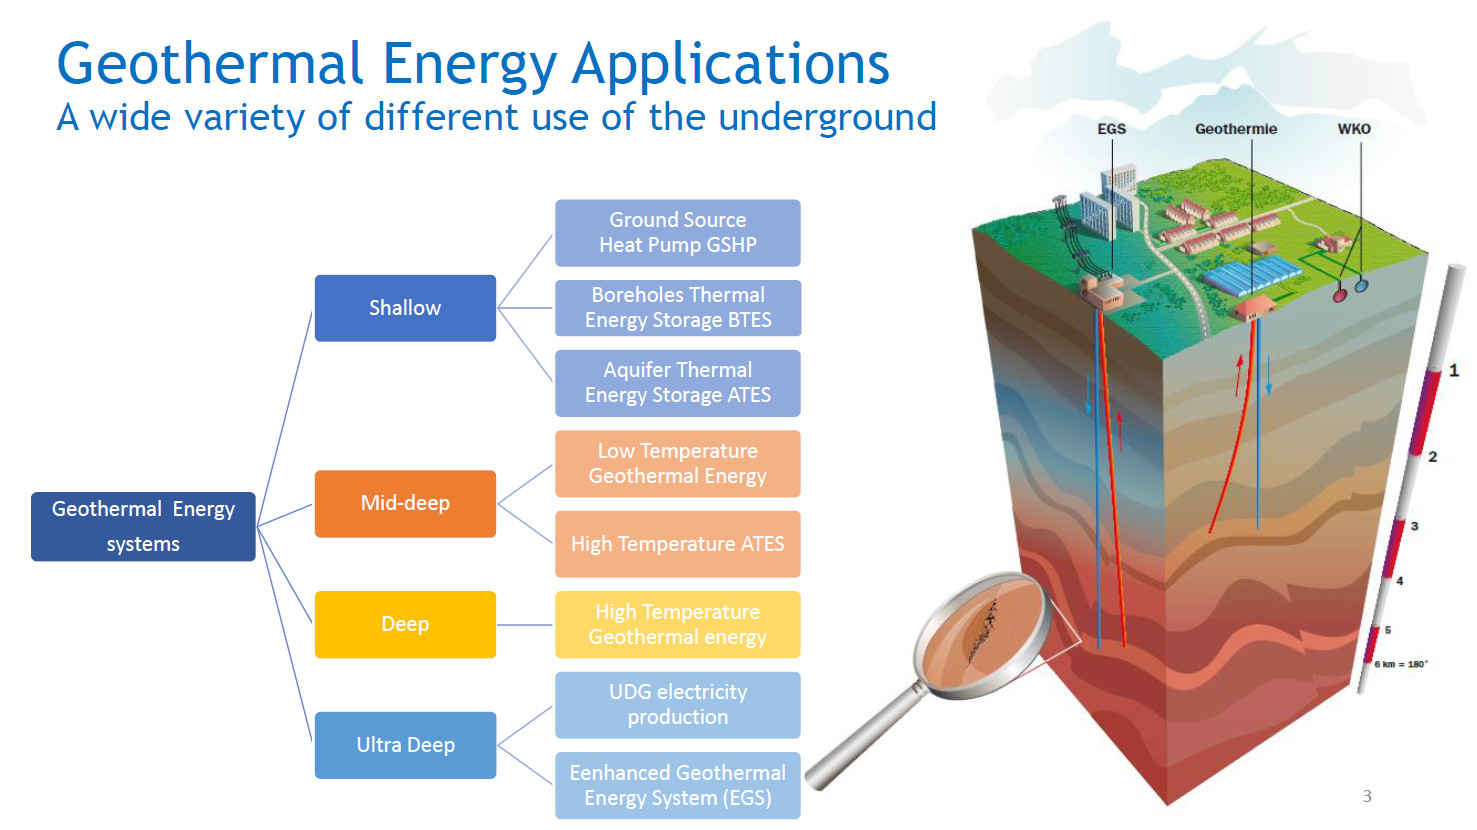
\includegraphics[width=.5\textwidth]{img/energie/geothermie-applications}

\paragraph{Aardwarmte}
De kern van de aarde bevat een onuitputtelijke hoeveelheid warmte. Op 2  kilometer diepte heeft grondwater in Nederland al een temperatuur van meer dan 70 graden Celsius.

Aardwarmte of geothermie (Grieks geo, aarde en thermos, warmte) is thermische energie, warmte, uit de Aarde.

Geothermie is een duurzame warmtebron en een van de mogelijkheden om aardgas te vervangen. Een geothermiebron kan jaarlijks de warmte produceren voor circa 10.000 woningen, ongeveer 02,20 PJ/jaar (Bron: www.geothermie.nl) afhankelijk van de geologische situatie ter plekke van de boringen.

\paragraph{Pilot-project Zwolle}
Zwolle Noord blijkt redelijk kansrijk voor de realisatie van een geothermiebron. Woningcorporaties hebben de intentie uitgesproken om die warmte af te nemen.

In het kader van het Europees subsidieprogramma “Geothermica” heeft Nederland via TNO een aanvraag gedaan voor een onderzoeksproject “Result”. Dit subsidieprogramma is gericht op onderzoek naar het toepassen van slimme boortechnieken in zogenaamde marginale reservoirs geothermie. De voor-aanvraag is onlangs door de Geothermica-organisatie van de EU gehonoreerd. In 2021 zal de eerste boring plaatsvinden in de Dijkslanden in Zwolle. Na een succesvolle boring bij deze productieput zal een tweede boring uitgevoerd worden, de injectieput. In 2023 zou dan de eerste winning plaats kunnen vinden.

Een proefboring geeft zekerheid over de geologische omstandigheden en helpt om het bronvermogen van de locatie te bepalen. De zekerheid van het vermogen is van groot belang om de investeringsbereidheid in de ontwikkeling van een warmtenet.

\paragraph{VERKLARINGEN, INSTANTIES, ADVIESBUREAUS}
SCAN    Seismische Campagne Aardwarmte Nederland

DAGO    Dutch Association Geothermal Operators

EBN    Energie Beheer Nederland

SodM    Staatstoezicht op de Mijnen

TNO    Nederlands Instituut voor Toegepast Natuurwetenschappelijk Onderzoek

Firan    Ontwerpt, realiseert, financiert en beheert toekomstbestendige energie-infrastructuur

IF Technology    Adviesbureau Geothermie, Bodemenergie , Aquathermie

Geotherm Energy Systems    Pionier op het gebied van bodemenergie en WKO

CE Delft        Onderzoeks- en adviesbureau op het gebied van milieu- en duurzaamheidsvraagstukken

Kas als Energiebron    Streeft ernaar het aantal gerealiseerde projecten per jaar te vergroten

Stichting Warmtenetwerk

Platform Geothermie

Masterplan Aardwarmte
\end{overwegingen}

\begin{aanbevelingen}
Toepassing van aardwarmte In de glastuinbouw is succesvol gebleken. In combinatie met ondergrondse opslag van CO2 en Warmte-Koude Opslag in de omgeving van glastuinbouwgebieden, zoals het Westland, betekent dat een enorme energiebesparing in vergelijking met confessionele methoden.

Het project in Zwolle betreffende toepassing van geothermie voor de verwarming van woonwijken zal kennis en ervaring opleveren voor bredere toepassing in Nederland.  Het SCAN-onderzoek dat momenteel gaande is zal uit  kunnen wijzen waar geothermie verder geschikt is voor bestaande en nieuwe woonwijken. De ontwikkelingen nauwgezet in de gaten houden. Aan de huidige boortechnieken en recente kennis en onderzoek zal het niet liggen hoe snel een en ander bredere toepassing vindt. Het SCAN-onderzoek loopt nog. Het is veeleer een organisatie-vraagstuk en het nemen van verantwoordelijkheden. Er is een fase van onderzoek en het verrichten van boringen met de nodige financiele risico’s en daarna aanleg, beheer en onderhoud van het leidingen-netwerk. 

Woningcorporaties willen wel meedoen, maar willen dan wel de zekerheid hebben dat er garanties zijn voor warmtelevering, anders kiezen ze voor warmtepompen en koude-warmte opslag per woning of woningblok. In het laatste geval behouden ze zelf de regie.
\end{aanbevelingen}

\paragraph{Literatuur}
Zwolle geeft energie, plan van aanpak 2018-2022

Voortgang geothermie, informatienota voor de raad, van Zwolle, januari 2020

De Bosatlas van de Energie, Noordhoff  Uitgevers Groningen

De Bosatlas van de Duurzaamheid, Noordhoff Uitgevers, Groningen

https://www.geothermie.nl

https://www.rijksoverheid.nl/onderwerpen/duurzame-energie/aardwarmte

https://www..iftechnology.nl/geothermie

https://vito.be/nl/diepe-geothermie

https://www.kasalsenergiebron.nl/duurzame-energie/aardwarmte

Wikipedia: Geothermie en Ile-de-France

La Geothermie a Villages Nature Paris (videofilms)

De Geo, Aarde, Klimaatvraagstukken, Studieboek VWO, ThiemeMeulenhoff, Amersfoort
\end{voorstel}
